\begin{defi}\label{def:dominant-weight}
 Let $\lambda$ be a weight of a representation of a Lie group with
 Weyl group $W$. Then \Dfn{$\dom_W(\lambda)$} is the unique
 dominant representative of the $W$-orbit $W\lambda$.
\end{defi}
\begin{exam}
 The Weyl group of $\SL(n)$ is the symmetric group $\fS_n$. Thus,
 $\dom_{\fS_n}$ returns its argument sorted into decreasing order.
\end{exam}
\begin{exam}
 The Weyl group of $\Sp(2n)$ is the hyperoctahedral group $\fH_n$ of
 signed permutations of $\{\pm 1,\dots,\pm n\}$. Thus, the dominant
 representative $\dom_{\fH_n}(\lambda)$ of a weight $\lambda$ is
 obtained by sorting the absolute values of its entries into
 decreasing order.
\end{exam}

We can now define the local rule.
\begin{defi}\label{def:local-rules}
 Let $A$ be a crystal and $B$ and $C$ be crystals of minuscule
 representations. Then the \Dfn{local rule}
 \[
 \tau^A_{B,C}\colon A\otimes B\otimes C \rightarrow A\otimes
 C\otimes B
 \]
 is an isomorphism of crystals defined for highest weight words
 $a\,b\,c$ as follows: let $\kappa$ be the weight of $a$, let
 $\lambda$ be the weight of $a\,b$ and let $\nu$ be the weight of
 $a\,b\,c$. Then
 \[
 \tau^A_{B,C}(a\,b\,c)= a\,\hat c\,\hat b,
 \]
 where %
 \[
 \hat c = \mu-\kappa\quad\text{and}\quad \hat
 b=\nu-\mu\quad\text{with}\quad\mu = \dom_W(\kappa+\nu-\lambda).
 \]
 We represent this by the following diagram:
 \begin{equation}\label{eq:local}
 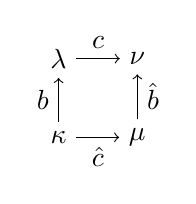
\begin{tikzpicture}[scale=1,baseline=(current bounding box.center)]
 \node (ka) at (0,0) {$\kappa$};
 \node (la) at (0,1) {$\lambda$};
 \node (nu) at (1,1) {$\nu$};
 \node (mu) at (1,0) {$\mu$};
 \draw[->] (ka) -- (la) node [midway, left] {$b$};
 \draw[->] (mu) -- (nu) node [midway, right] {$\hat b$};
 \draw[->] (la) -- (nu) node [midway, above] {$c$};
 \draw[->] (ka) -- (mu) node [midway, below] {$\hat c$};
 \end{tikzpicture}
 \end{equation}
 Since any isomorphism between crystals is determined by specifying
 a bijection between the corresponding highest weight words, this
 definition can be extended to an isomorphism between
 $A\otimes B\otimes C$ and $A\otimes C\otimes B$ by applying the
 lowering operators.
\end{defi}
\begin{rema}
\looseness-1
 When $B=C$ is the crystal associated with the vector representation
 of $\SL(n)$, the local rule~\eqref{eq:local} is Fomin's for
 Schützenberger's jeu de taquin~\cite[A~1.2.7]{MR1676282}. More
 explicitly, if $\lambda$ is the only partition of its size that
 contains $\kappa$ and is contained in $\nu$, then $\mu=\lambda$.
 Otherwise there is a unique such partition different from
 $\lambda$, and this is $\mu$.
\end{rema}

\begin{rema}\label{rmk:symmetry-of-local-rule}
 As in the classical case the local rule is symmetric in the sense
 that $\mu = \dom_W(\kappa+\nu-\lambda)$ if and only if
 $\lambda = \dom_W(\kappa+\nu-\mu)$, see
~\cite[Lem.~4.1.2]{MR1661263}.
\end{rema}
